\section {Arhitectura sistemului}

Sistemul prezentat presupune atât o partare hardware, cât 'si una software. Hardwareul realizează adaptarea dintre terminalul analog \acrshort{pots} 'si placa digitală de dezvoltare Raspberry Pi, iar ca software am folosit NodeJS pentru server 'si Android pentru a implementa un client al serverului.

Cu ajutorul multimetrului am dedus schema electrică a tastaturii 'si am găsit contactele care sunt conectate în cazul apăsării butonului de pe ultimul rând, coloana din mijloc. Scurtcircuitarea contactorului lamelar care depistează ridicarea receptorului 'si legarea la difuzorul terminalului au fost realizate mai u'sor, circuitul fiind parcurs vizual.

\begin{figure}[h!]
  \centering
  \fbox {
    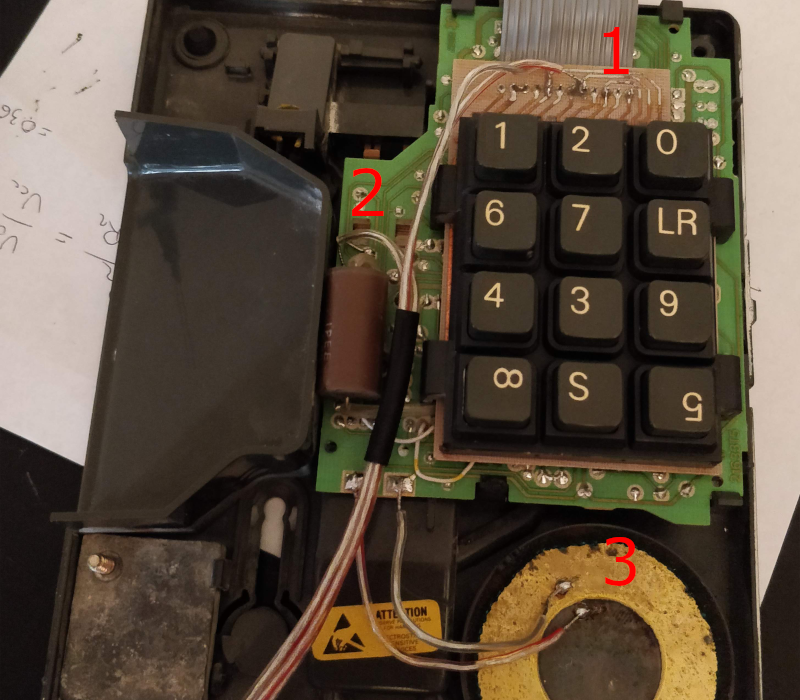
\includegraphics[width=\singlephoto]{04/11_terminal_pots.png}  
  }
  \caption{Depanare 'si interfa'tare terminal POTS}
  \medskip
  \small
  1 - contacte buton deschidere, 2 - contactor lamelar receptor, 3 - contacte difuzor
\end{figure}


\subsection {Raspberry Pi HAT}

După ce etapa de prototipare pe breadboard a fost finalizată, am transcris schema electrică a circuitului cu ajutorul softwareul Fritzing. Proiectarea unui 
\acrfull{pcb} reprezintă penultimul pas înainte de etapa de produc'tie în masa. Printre parametrii importan'ti în deciderea designului unui circuit printat se numără:

\begin{itemize}
  \item Tehnologia de montare a componentelor pe \acrshort{pcb} (\acrfull{tht} sau \acrfull{smd})
  \item Numărul de straturi de circuit (alegeri comune sunt 2, 4, însă dispozitive complexe precum plăcile video pot folosi până la 12 straturi)
  \item Grosimea 'si culoarea plăcii de fibra de sticlă
  \item Lă'timea unui traseu pe placă
  \item Distan'ta minima intre trasee
  \item Diametrul via-urilor (găuri verticale în placă folosite pentru a conecta straturile)
  \item Materialul folosit pentru lipire 'si meterialul folosit pentru pinii de interfa'tare
\end{itemize}

Pentru a realiza un \acrfull{hat} compatibil cu Raspberry Pi, am folosit softwareul Fritzing. Acesta permite proiectarea schemei electrice 'si ulterior trasarea conexiunilor pe layoutul fizic al plăcii. Considerand complexitatea redusă a proiectului, s-a ales folosirea configura'tiei implicite cu două straturi, împreună cu următorii parametri pe care i-am introdus în Fritzing ca 'si constrângeri de design:

\begin{figure}[h!]
  \centering
  \fbox {
    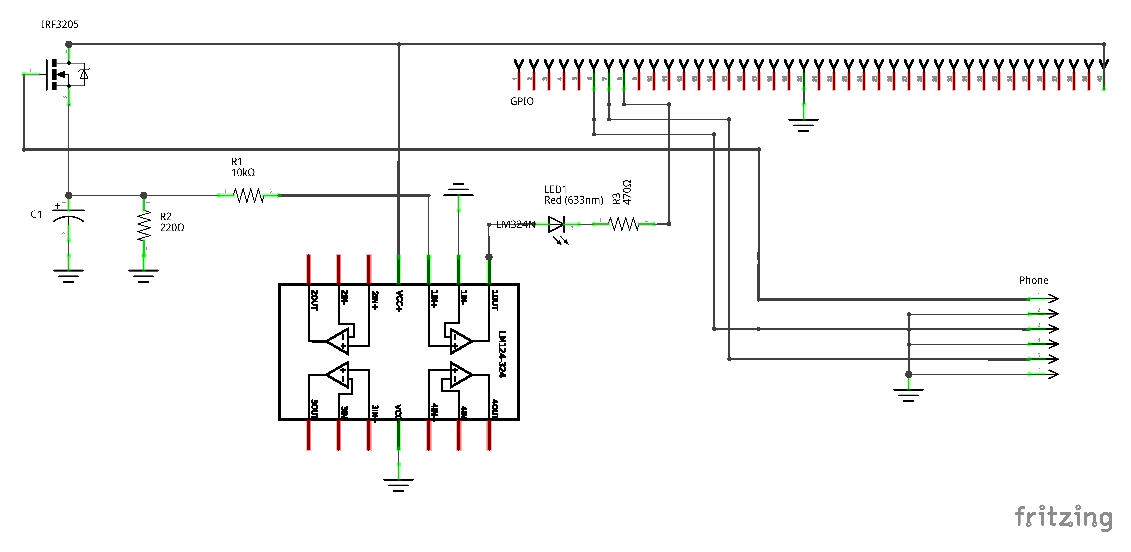
\includegraphics[width=\singlefigure]{04/04_schema_electrica_hut.pdf}  
  }
  \caption{Schema electrica HAT Raspberry PI}
\end{figure}

Ac'tionarea butoanelor terminalului \acrshort{pots} se realizează cu ajutorul unor opto-cuploare, izolând circuitul interfonului care este proiectat pentru a func'tionă cu spike-uri de până la 90V de circuitul Raspberry Pi.

Detectarea unui apel este realizata prin legarea unui \acrfull{mosfet} la bornele difuzorului terminalului \acrshort{pots} 'si înserierea cu un amplificator opera'tional în regim de comparator cu referin'tă de 0.1V. Am folosit de asemenea 'si un Filtru Trece Jos deoarece terminalul este sensibil la zgomote, declan'sând accidental notificarea.

\begin{figure}[h!]
  \centering
  \fbox {
    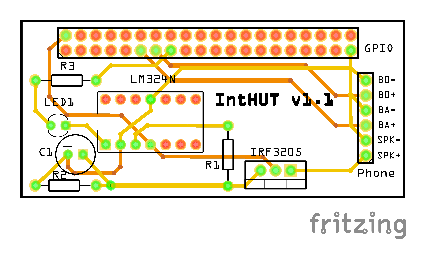
\includegraphics[width=\singlefigure]{04/05_schema_pcb_hut.pdf}  
  }
  \caption{Design \acrshort{pcb} HAT \\(galben - stratul de sus, portocaliu - stratul de jos)}
\end{figure}

\subsubsection {Optocuploare improvizate}

Datorită crizei globale de semiconductori, o plăcu'tă breakout care include două optocuploare costă aproximativ 50 RON \cite{RoboFun2022}. Considerând simplitatea func'tionarii acestui circuit, am decis să construiesc propria solu'tie, folosind componetele de bază: un rezistor pentru limitat curentul, un LED 'si un fotorezistor. Platforma Raspberry Pi furnizează pinilor sai \acrshort{gpio} 3.3V 'si un curent maxim de 16mA, iar un LED ro'su are o cădere de tensiune de 2.4V:

\begin{equation}
\label{eq:test}
\begin{split}
I_{GPIO} & =10\ mA=10^{-2} A\\
V_{R} & =V_{GPIO} -V_{LED} =3.3V-2.4V=0.9V\\
I_{GPIO} & =\frac{V_{R}}{R} \ sau\ R=\frac{V_{R}}{I_{GPIO}} =\frac{0.9V}{10^{-2}A} =90\Omega
\end{split}
\end{equation}

Am lipit rezistorul de 90$\Omega$ la anodul ledului 'si am încastrat LED-ul împreună cu fotorezistorul într-o incintă fără lumină.

\begin{figure}[!ht]
\begin{center}
  \subfloat[Schema optocuplor \cite{OptocouplerCircuitsToday}]{\label{fig:optoa}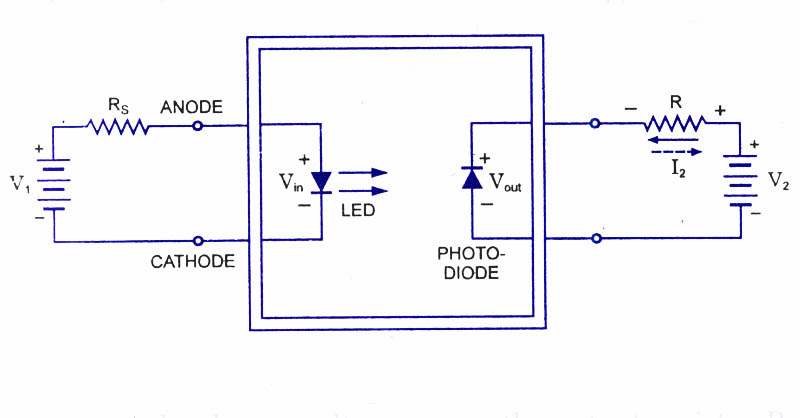
\includegraphics[width=\doublefigure]{04/01_optocoupler_scheme.jpg}}
  \hfill
  \subfloat[Componenta realizată manual]{\label{fig:optob}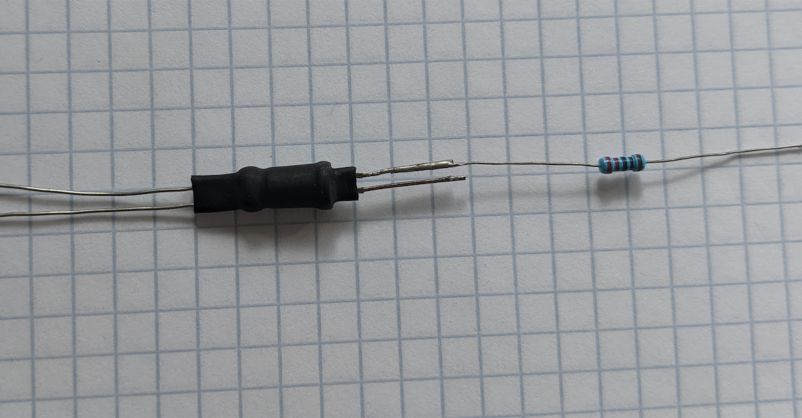
\includegraphics[width=\doublefigure]{04/02_optocoupler_assembly.png}}
  \caption{Schema electrică optocuplor (a) 'si rezultat ansablu (b)}
  \label{fig:opto}
\end{center}
\end{figure}


Deoarece aveam nevoie să scurtcircuitez un contactor pe partea terminalului \acrshort{pots} am omis rezisten'ta legată fotorezistorului. Atunci când ledul este aprins, rezisten'ta fotorezistorului scade, comportandu-se aproape că un conductor ideal, atingând lamelele contactorului corespunzător receptorului.

După ce toate traseele au fost plasate, ultimul pas este umplerea spa'tiului rămas pe fiecare strat cu un plan legat la GND pentru a reduce emisiile electromagnetice. Înainte de a trimite fi'sierul Gerber spre a fi produs, am folosit constrângerile definite ini'tial pentru a valida proiectul, asigurandu-ne că acesta poate fi produs în realitate.

\begin{table}[ht!]
\begin{tabular}{llllll}
\hline
Nr. &  &  & Lă'time & Diametru & Material \\ 
straturi & Tehnologie & Grosime & traseu & via & finisaj \\
\hline
\hline
2 & \acrshort{tht} & 1.6mm & 1mm & 0.5mm & LeadFree HASL-RoHS\\
\hline
\end{tabular}
\centering
\caption{Parametri ale'si pentru fabricarea \acrshort{pcb}}
\label{tab:params}
\end{table}

\begin{figure}[!ht]
\begin{center}
  \subfloat[Vedere din fata \acrshort{pcb}]{\label{fig:hata}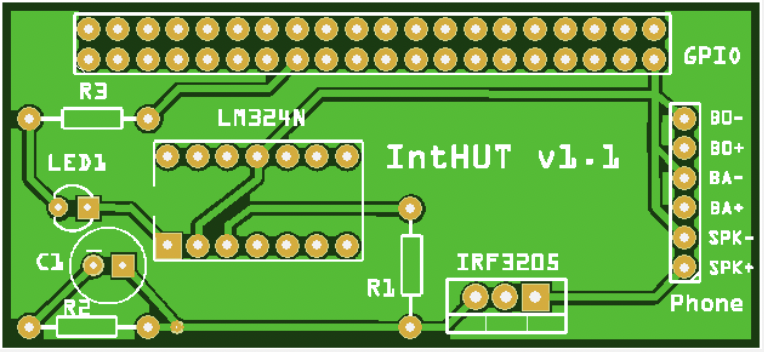
\includegraphics[width=\doublefigure]{04/06_pcb_front.png}}
  \hfill
  \subfloat[Vedere din spate \acrshort{pcb}]{\label{fig:hatb}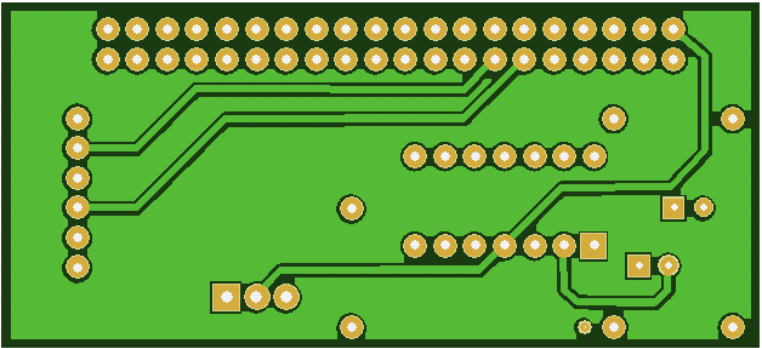
\includegraphics[width=\doublefigure]{04/06_pcb_back.png}}
  \caption{Randare plăcuta înainte de comandat}
  \label{fig:hat}
\end{center}
\end{figure}

\subsection {Webserver NodeJS}

NodeJS este un mediu de rulare JavaScript asincron, cu un design centrat în jurul unei bucle de evenimente. Este proiectat pentru realizarea aplica'tiilor scalabile ce folosesc re'teaua. \cite{NodeJs2021}

\begin{figure}[H]
  \centering
  \fbox {
    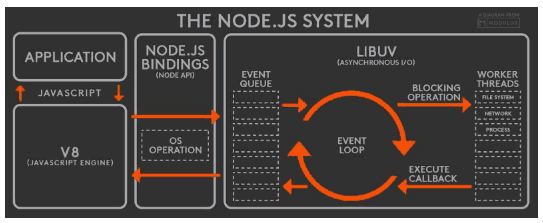
\includegraphics[width=\singlefigure]{04/12_node_js_system.png}  
  }
  \caption{Ilustrare event loop 'si callback queue \cite{DevelopPaper2019}}
\end{figure}

Pentru a în'telege cum rulează codul javascript în acest mediu de rulare, trebuie să ne familiarizăm cu modeul de asincroneitate pus la dispozi'tie, care diferă semnificativ de cel multi-threadded. Codul JavaScript este parcurs cu ajutorul engine-ului V8 'si este tradus în apeluri la librăria nativă libuv care se va ocupa de executarea lor plasarea în coada de evenimente. Atunci când "libuv" are nevoie să facă un apel sincron de sistem, precum interogarea unui server DNS, o face prin intermediul unui thread-pool, ata'sând un callback pentru a fi chemat atunci când este gata.

\subsubsection {Criptare HTTPS}

Conform cerin'telor func'tionale, canalul de comunicare dintre client 'si server trebuie să fie securizat cu un protocol \acrfull{https} pentru a permite trimiterea credentialelor fără a fi susceptibile la atacuri de tip \acrfull{mitm}. S-a ales folosirea Let's Encrypt, un serviciu gratuit pentru emiterea unui certificat semnat de o autoritate reputabila.

Pentru a verifica identitatea serverului, clientului îi este cerut să afi'seze un 'sir de date la o rută statică prestabilită, dovedind astfel autoritate asupra serverului căruia i se va emite certificatul. După completarea acesor pasi 'si emiterea certificatului, configurarea serverului să implementeze protocolul \acrshort{https} este relativ simpla:

\begin{figure}[H]
  \centering
  \fbox {
    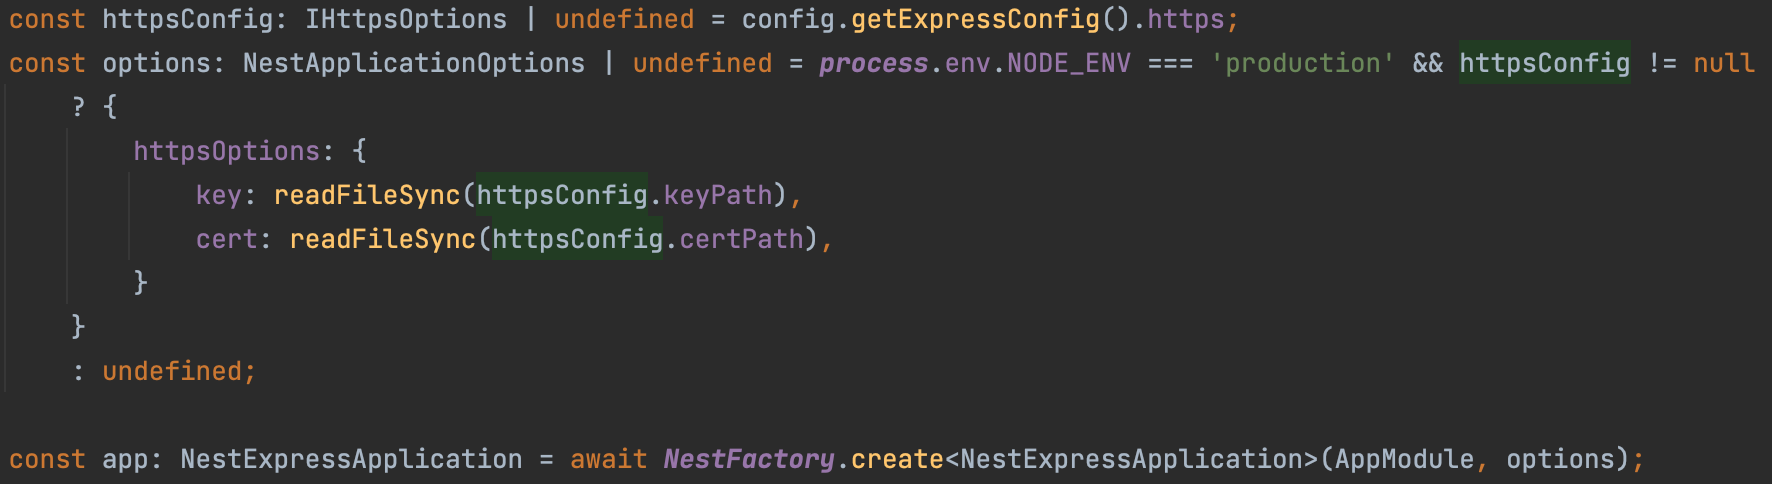
\includegraphics[width=\singlefigure]{04/13_configurare_ssl.png}  
  }
  \caption{Configurare aplica'tie NestJs pentru a folosi certificate}
\end{figure}

Este de men'tionat că începând cu versiunea de Android 9 (Pie) ca parte dintr-o ini'tiativă de mărire a securită'tii, sistemul de operare va bloca conexiunile PLAINTEXT dacă aplica'tiile nu configurează o excep'tie pentru server \cite{Digicert2018}. De asemenea, prezentarea unor certiifcate self-signed sau insuficiente informa'tii vor produce rezultate similare, fiind nevoie ca serverul să prezinte întregul lan't de certificate (al serverului, ale autorită'tilor intermediare 'si în final cel al autorită'tii centrale). 

\subsubsection {Autentificare}

Pentru autentificarea 'si validarea credentialelor utilizatorilor, am ales metoda \acrfull{jwt}, un standard open source în industrie conform RFC 7519. În cea mai compactă formă a sa, acesta este compus din trei păr'ti, despăr'tite prin caracterul ".":

\begin{enumerate}
  \item Header (algoritm 'si tipul tokenului)
  \item Con'tinut (id utilizator, nume, rol)
  \item Semnătură
\end{enumerate}

Semnătura este calculată cu ajutorul unui algoritm simetric de hashing \acrfull{hs256} 'si a unei chei private aplicat pe forma codată în baza 64 a con'tinutului 'si metadatelor despre token (expirare, emi'tător, audien'tă, subiect). Toate cele trei informa'tii sunt apoi concatenate cu caracterul "." între, constituind forma finală ce va trimisă clientului. Clientul va transmite acest token în comunica'tiile ulterioare cu serverul, acesta folosindu-se de mesaj, semnătură 'si cheia privată pentru a determina dacă a fost sau nu modificat pe parcurs.

Folosirea algoritmului simetric implica faptul că secretul este utilizat atât pentru generarea de tokenuri, cât 'si pentru validarea lor. În cazul aplica'tiei din lucrare, aceasta nu este o problemă, deoarece ambele metode rulează în interiorul aceluia'si proces, fară să expună aplica'tia la vulnerabilită'ti.

Un avantaj al \acrshort{jwt} este faptul că serverul nu trebuie să între'tină starea unei tabele de sesiuni a utilizatorilor. În esen'tă daca un utilizator este în posesia unui token ne-expirat, aceste este considerat autentificat. Prin urmare, mai multe instan'te ale serverului pot valida în paralel identitatea utilizatorilor, fară nevoia de a interoga o baza de date sau o memorie cache partajată, permi'tând astfel scalarea pe orizontală a aplica'tiei.

\subsubsection {NestJS}

Construit peste cel mai popular framwork pentru aplica'tii web disponibil pentru Node.js, NestJS îmbunătă'te'ste experien'tă dezvoltării serviciilor web folosind func'tii experimentale din Typescript care permit interpretarea la transpilare a decoratorilor pentru metode 'si clase. De asemenea urmăre'ste un design \acrshort{mvc} 'si are pachete între'tinute oficial pentru taskuri comune, cum ar fi conectarea la o bază de date sau proiectarea unui mecanism de autentificare 'si verificare a identiatii utilizatorilor.

\subsubsection {Mutex}

Din natura asincronă a limbajului 'si posibilitatea sistemului de a avea mai mult de un utilizator, trebuie luat în considerare cazul în care mai mul'ti utilizatori încearcă să interac'tioneze cu sistemul în acela'si timp. A'sadar, trebuie implementat un mecanism similar semaforului binar, numit mutex. Diferen'tă dintre acestea fiind că în cazul mutexului, doar de'tinătorul original poate să îl elibereze spre a fi folosit din nou.

Acest comportament este dorit pentru a informa clien'tii serviciului în cazul în care requestul nu poate fi satisfăcut deoarece resursa este ocupată de altcineva.

\begin{figure}[H]
  \centering
  \fbox {
    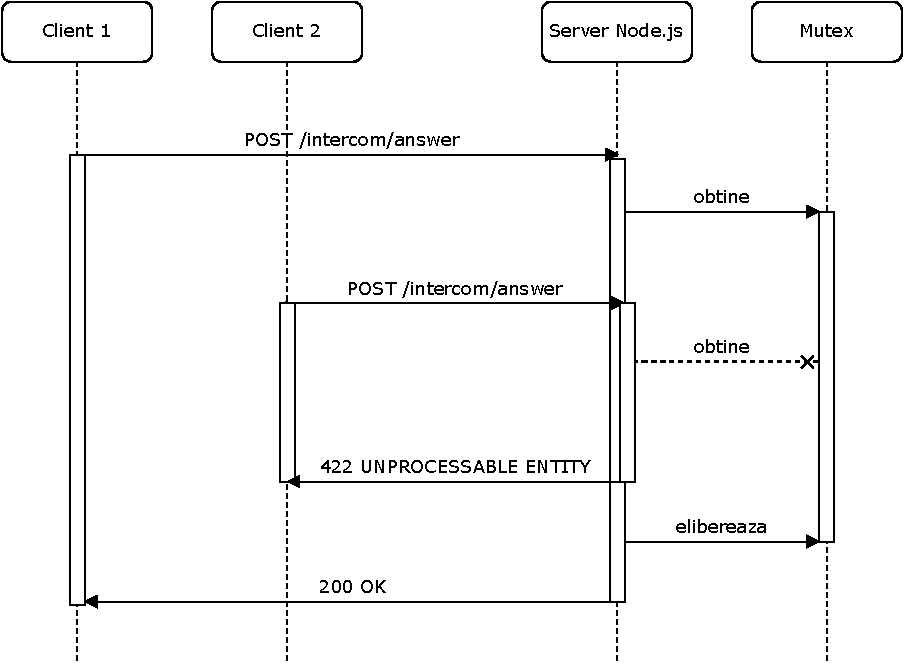
\includegraphics[width=\singlefigure]{04/03_mutex_diagram.pdf}  
  }
  \caption{Ilustrare resursă disputată între doi utilizatori}
\end{figure}


\subsubsection {Validarea entită'tilor}

Folose'ste func'tii din Typescript 'si NestJS pentru a adaugă 'si citi metadate prin intermediul decoratorilor de metode. \acrfull{dto} este reprezentarea unui model din baza de date, dar encodat favorabil pentru interpretarea u'soară a clien'tilor. Majoritar, acesta va con'tine mai pu'tine câmpuri decât exista în baza de date (reprezentarea unui utilizator nu va avea câmpul pentru parola).

Câmpurile unui \acrfull{dto} sunt adnotate cu tipul a'steptat la runtime, 'si printr-un interceptor de nest care rulează atunci când este invocată metoda unui controller \acrshort{rest}, obiectul primit că parametru este verificat contra specifica'tiilor din metadate. În cazul în care validarea e'suează, clientului îi este întors status 400 (Bad Request) indicând o eroare de formatare a requestului.

Mutând responsabilitatea verificării entită'tilor în cadrul serverului, se mitigheaza 'si lipsa unei scheme la nivelul bazei de date, inerente solu'tiilor NoSQL. Prin urmare se reduce riscul unor inconsisten'te în datele stocate.

\subsubsection {Roluri}

Urmărind re'teta de dezvoltare observată în validarea entită'tilor, am creat un mecanism de adăugare a metadatelor pe rutele controllerelor in vederea implementarii rolurilor utilizatorilor.

Partea de verificare a unui user în timpul unui request, revine a'sa-numitelor Guard-uri care implementează o interfa'tă comună. În cazul vederilor pentru aplica'tia de admin dorim să restrictionam afi'sarea să utilizatorilor normali, a'sadar înlăn'tuim Guard-urile ce garantează autentificarea unui utilizator 'si rolul de administrator. În cazul în care un user nu este administrator, acestuia i se întoarce un cod de status 403 (Forbidden) - serverul a autentificat utilizatorul, dar acesta nu are suficiente permisiuni pentru a accesa resursa.

\subsubsection {Documenta'tie}

Într-un proiect de lungă durată, documenta'tia joacă un rol esen'tial în u'surin'ta de mentenan'tă 'si dezvoltare a codului. Despăr'tirea logică a componentelor aplica'tiei cât 'si explicarea eventualelor căi logice 'si răspunsuri posibile ajută atât clien'tii externi consumatori ai \acrshort{api}-ului cât 'si dezvoltatorii noi care încearcă să introducă primele modificări.

Astfel, am ales Swagger pentru a parcurge proiectul 'si genera pagini de documenta'tie pentru toate rutele serviciului \acrshort{rest}, împreună cu comentarii 'si poten'tiale status code-uri la care trebuie să se a'stepte clien'tii. De asemenea, Swagger include 'si un client \acrshort{rest} în pagină, împreună cu schema obiectelor 'si tipurile de date a'steptate nu lasă loc de interpretat în comportamentul serverului.

\begin{figure}[H]
  \centering
  \fbox {
    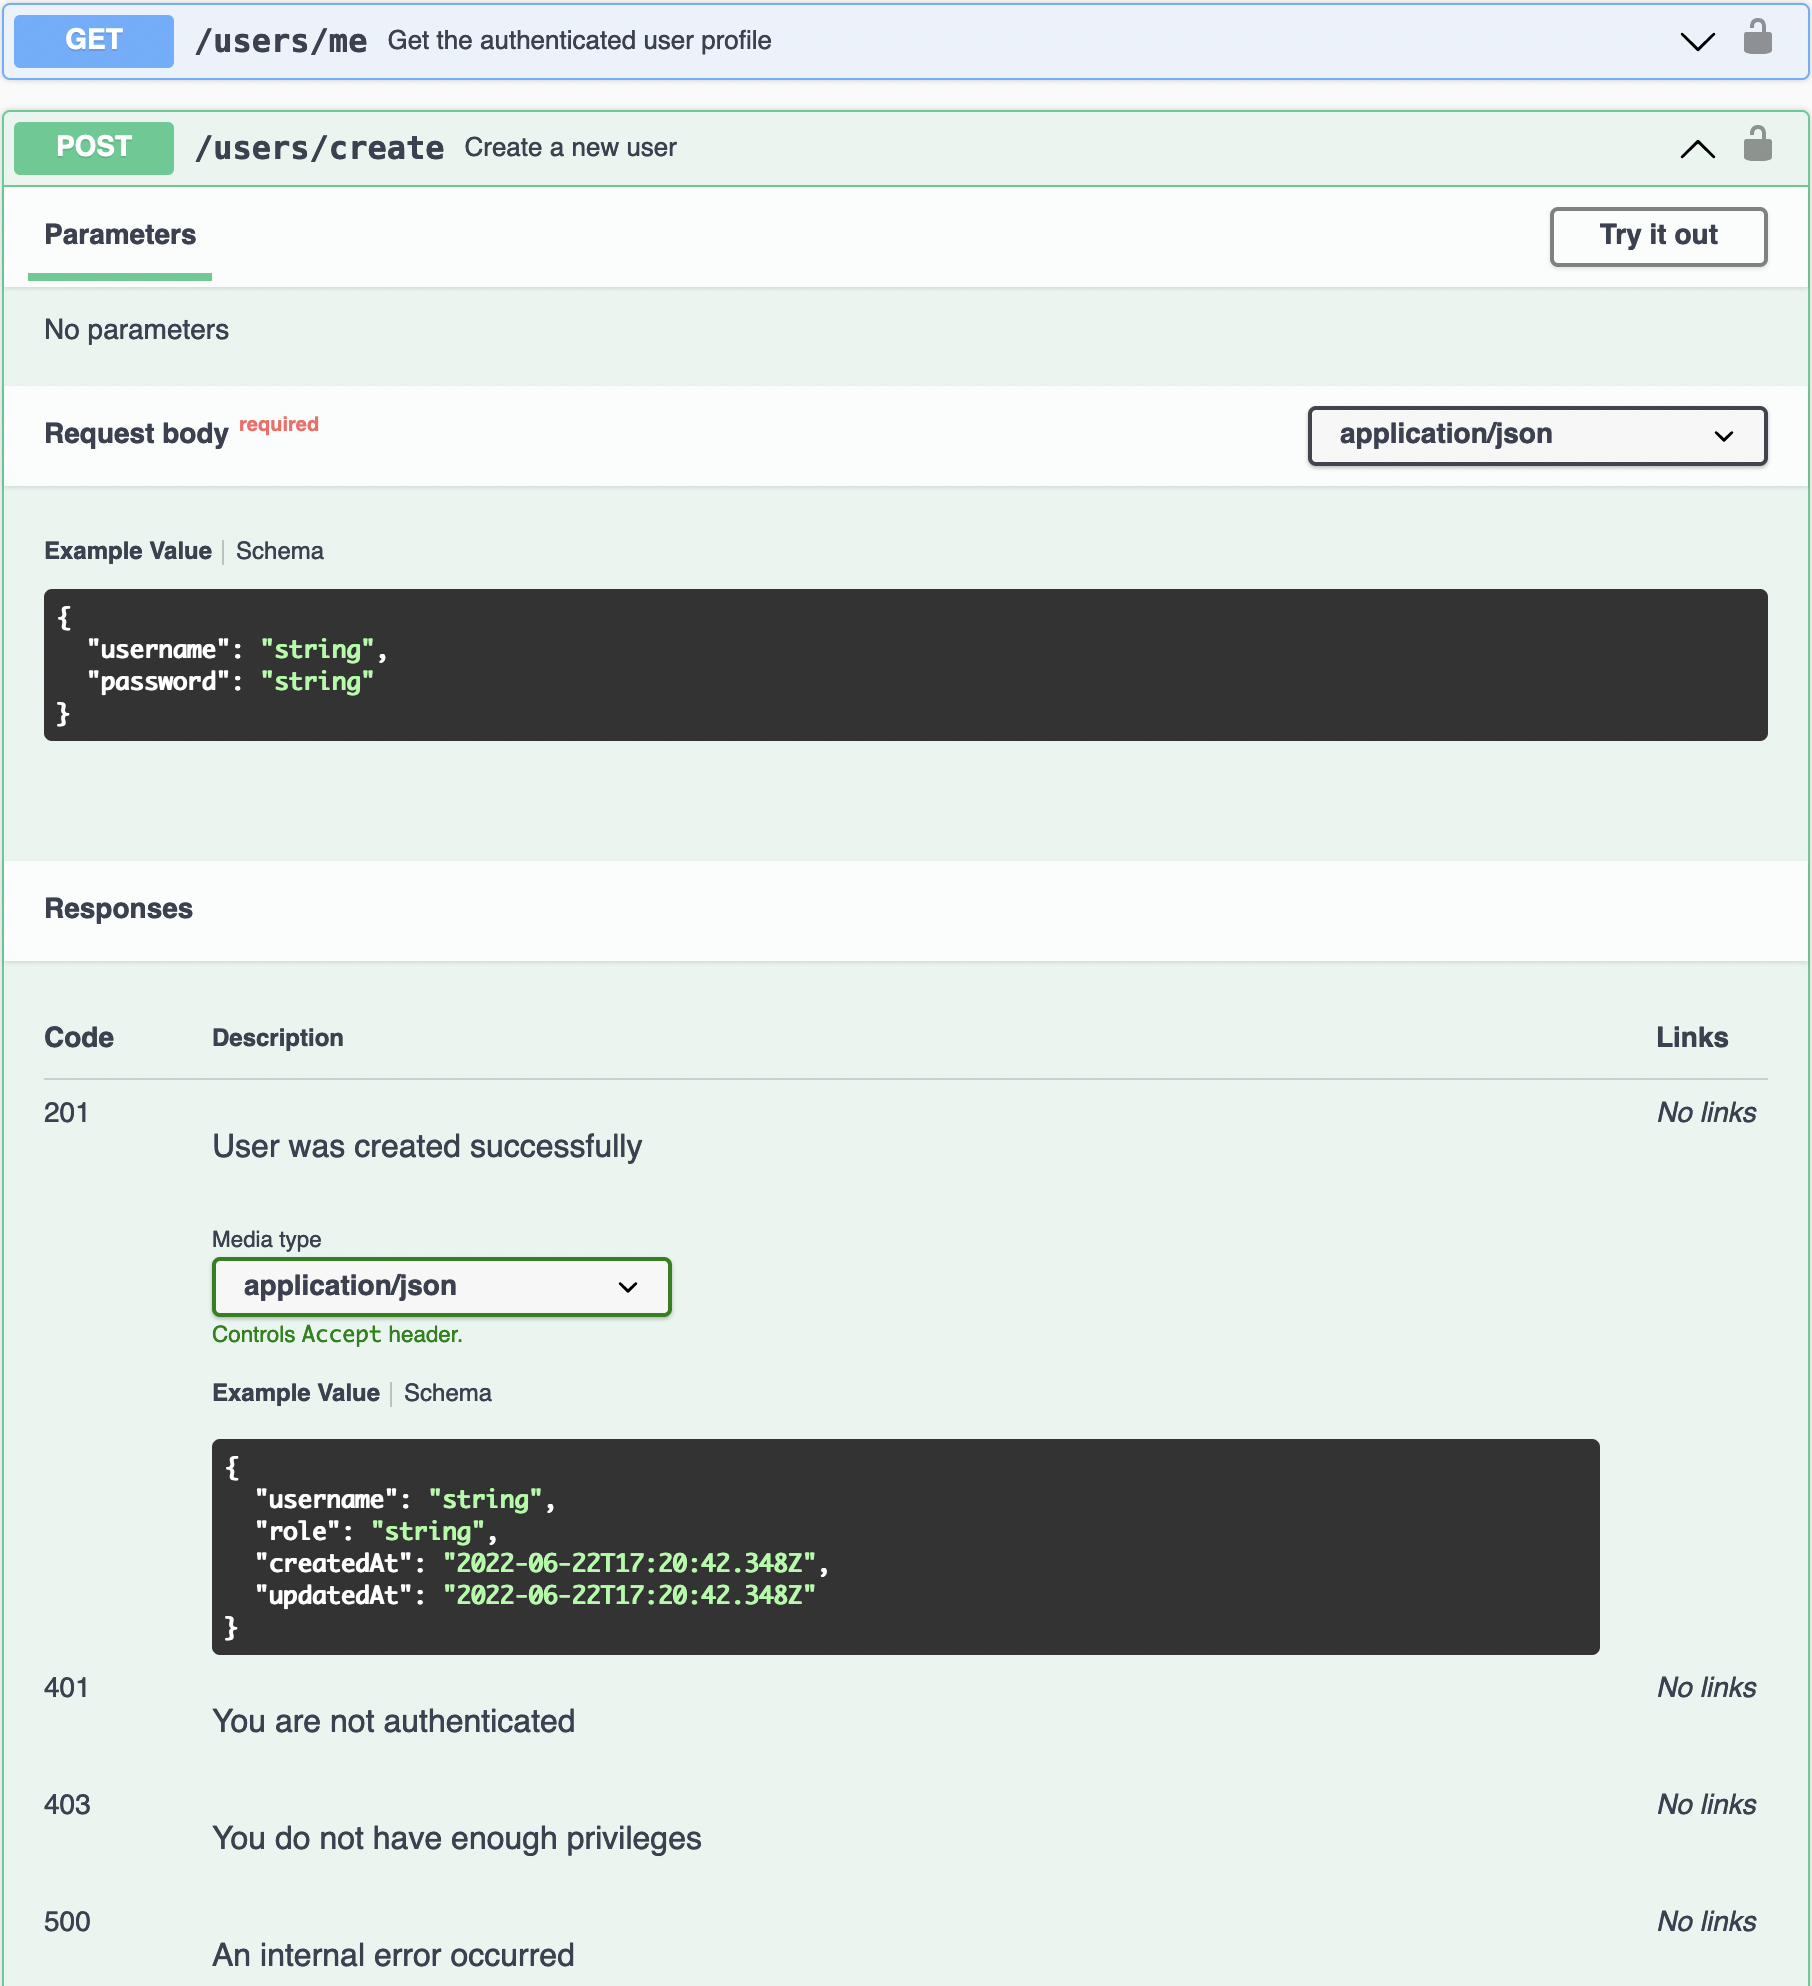
\includegraphics[width=\singlephoto]{04/10_swagger_doc.png}  
  }
  \caption{Documenta'tie generată pentru ruta /users/create}
\end{figure}

\subsection {Android}

Android este o platformă mobilă care s-a maturizat pe parcusul a 12 versiuni majore 'si principalul competitor de pia'tă al iOS. Im dezvoltarea acestei aplica'tii am folosit o abordare similara cu cea a serverului, fiind organizată într-un pattern de design \acrshort{mvc}. O aplica'tie Android poate fi alcătuită din mai multe componente cu roluri specifice: Activity, Service 'si BroadcastReceiver. Fiind un sistem de operare care vizează dispozitivele mobile, este optimizat pentru folosirea eficientă a resurselor 'si a bateriei, astfel că folosirea incorectă a componentelor anterioare poate duce la oprirea accidentala a aplica'tiei sau a unui serviciu în timpul unor opera'tiuni importante.

O alta particularitate în programarea acestor aplica'tii este că desenatul interfe'tei 'si interceptarea evenimentelor de la utilizator se realizează într-o buclă pe firul de execu'tie principal. Astfel, orice opera'tiuni adi'tionale executate pe acest thread trebuie alese cu aten'tie pentru a nu duce la aparenta îngreunare prin introducerea laten'tei la afi'saj 'si la interpretat evenimente de input de la utilizator. Opera'tiuni care presupun a'steptarea după sisteme de \acrshort{io} precum un apel prin re'tea, sunt complet blocate din a fi executate pe threadul principal, aruncând o excep'tie numită "NetworkOnMainThreadException" \cite{AndroidNetwork2022}.

\subsubsection {Dependency Injection}

Pentru a gestionarea u'soară a modulelor aplica'tiei 'si diferitele surse de date, s-a ales folosesirea Dagger2, un framework bine cunoscut de Java. El vine cu extensii pentru Android ce permit controlul granular asupra instan'tierii modulelor necesare în func'tie de ciclul de via'tă al aplica'tiei sau al unui Activity. Astfel putem defini module globale, precum cel care cheamă api-ul web, instantiat o singură dată pe durata aplica'tiei, sau module locale, precum cel de SharedPreferences care se realoca de fiecare dată când se intră în ecranul principal.

Pe lângă organizarea proiectului în module logice în func'tie de func'tionalită'ti, Dagger ajută 'si la managementul memoriei într-un limbaj de programare cu Garbage Collector, precum Java, evitând alocări nenecesare sau frecvente.


\section {Implementarea sistemului}

\subsection {Server}

Chiar dacă autentificarea prin interfa'tă grafică de administrator beneficiază de acela'si standard de securitate că 'si ceilal'ti clien'ti, s-a ales crearea unui alt server pe un port diferit de cel al \acrshort{api}-ul, permi'tând flexibilitate maximă utilizatorului final în alegerea expunerii serviciilor.

Personal, am expus serviciul de API pe un port rutat public 'si interfa'tă pe un port privat, blocat din firewall. În esen'tă, orice utilizator normal poate interac'tiona cu sistemul atâta timp cât este autentificat, însă interfa'ta de administrare este disponibilă doar din interiorul re'telei din acasă.

\begin{figure}[H]
\begin{center}
  \subfloat[Strategie \acrshort{jwt} pentru autentificarea clien'tilor \acrshort{api}]{\label{fig:jwta}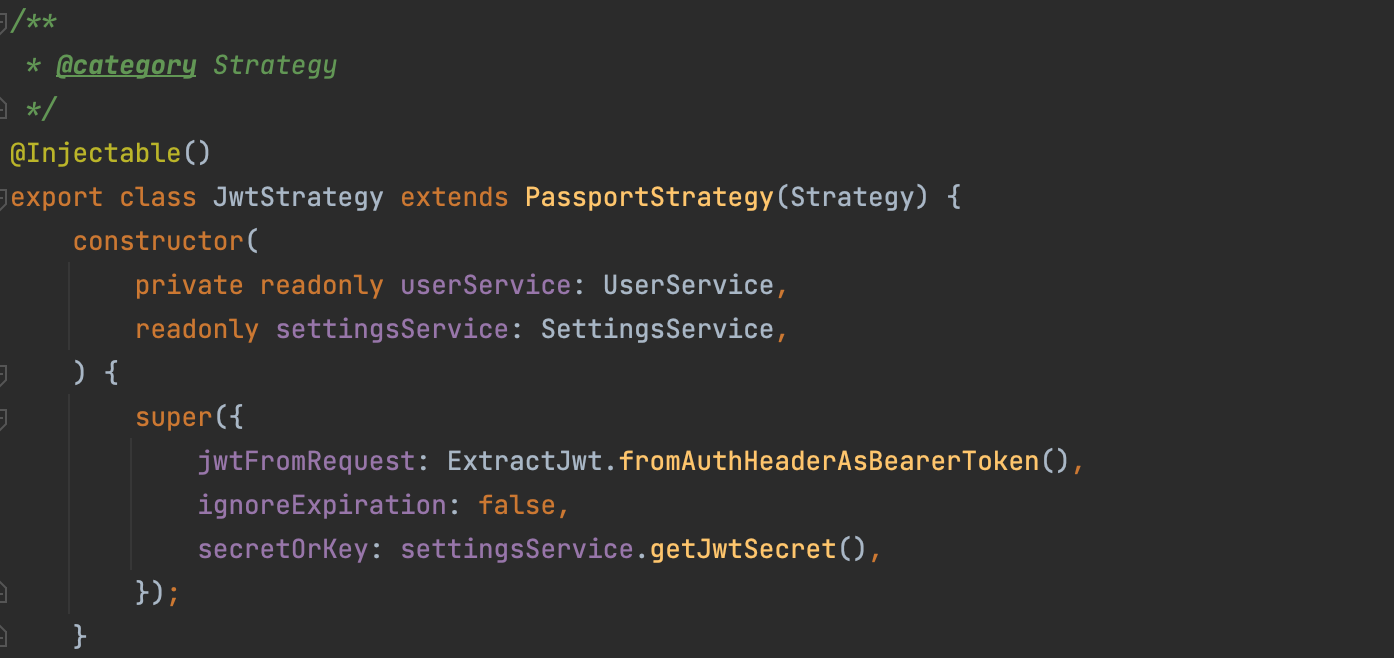
\includegraphics[width=\doublefigure]{04/15_node_jwt_api.png}}
  \hfill
  \subfloat[Strategie \acrshort{jwt} pentru autentificarea din browser, prin intermediul cookies]{\label{fig:jwtb}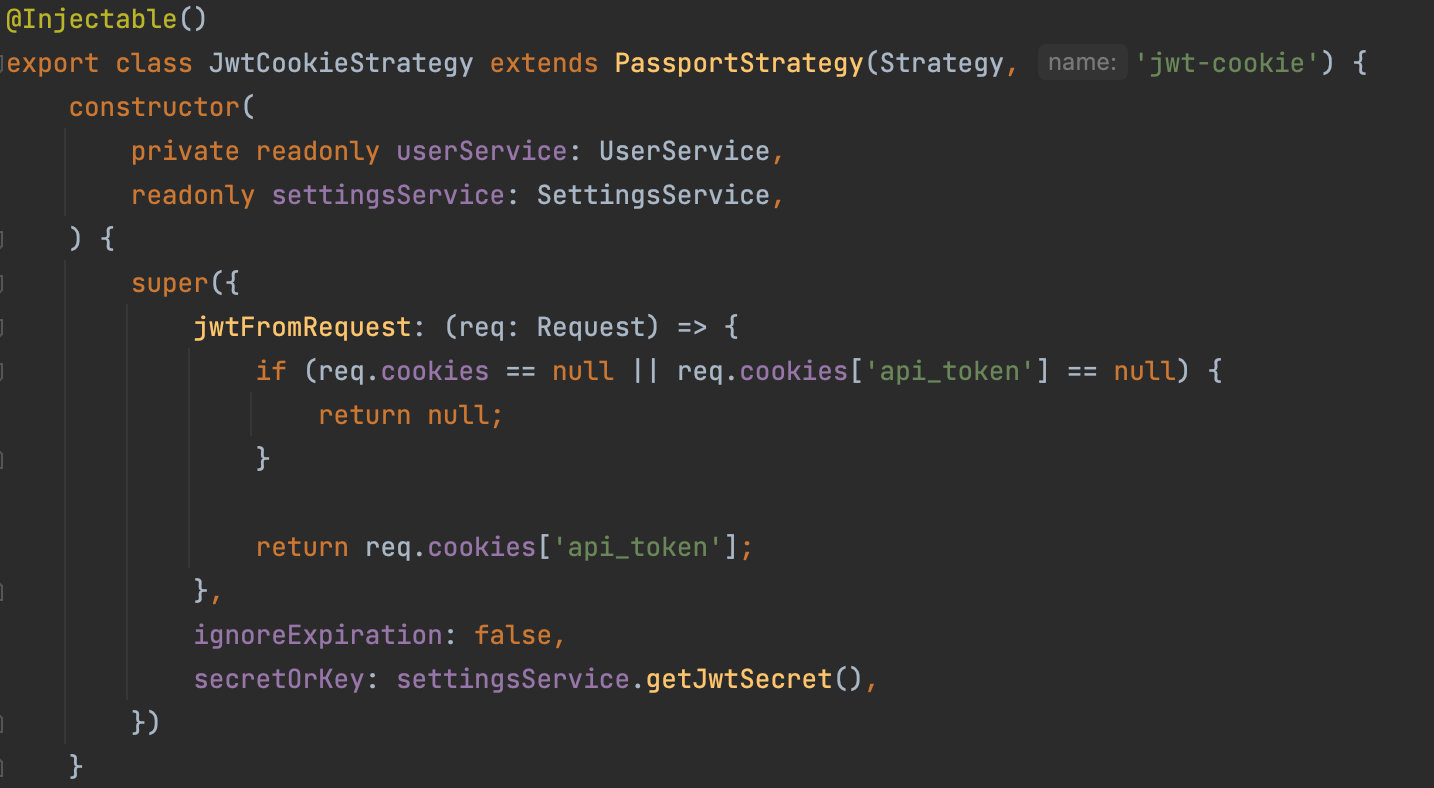
\includegraphics[width=\doublefigure]{04/16_node_jwt_cookie.png}}
  \caption{Implementare logica autentificare utilizatori}
  \label{fig:jwt}
\end{center}
\end{figure}

Secven'ta de generare a comenzilor pentru deschiderea interfonului se află în clasa IntercomService, această secven'tă include: ob'tinerea mutexului, ridicarea receptorului, a'steptarea pentru o secundă, apăsarea butonului pentru răspuns de două ori, cu o pauză de 1.2s între 'si în final eliberarea mutexului. Secven'tă pentru respingerea unui apel a fost implementată într-o manieră similară, presupunând doar ridicarea receptorului 'si închiderea sa după un interval prestabilit de timp.

\begin{figure}[H]
  \centering
  \fbox {
    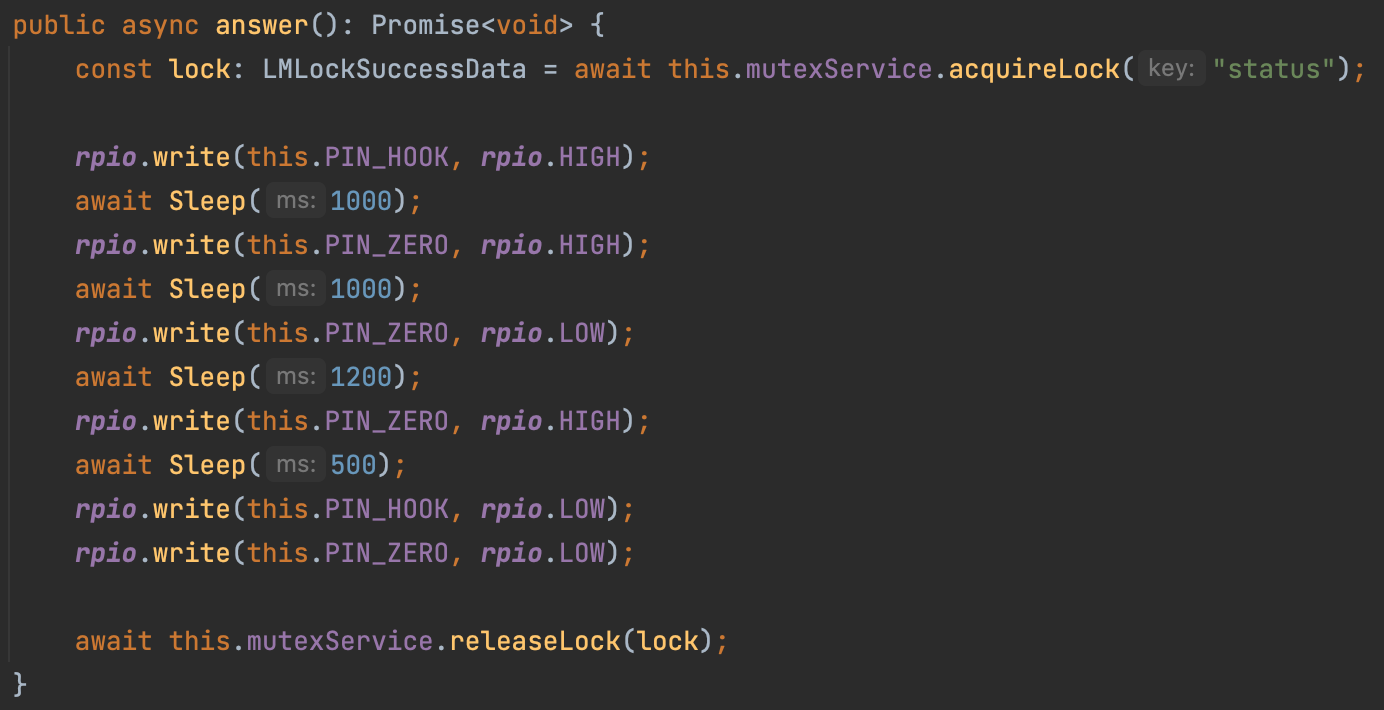
\includegraphics[width=\singlelongfigure]{04/09_serviciu_intercom.png}  
  }
  \caption{Implementarea metodei pentru permis accesul din IntercomService}
\end{figure}

Pentru statistici, metoda care persistă un Log în baza de date oferă utilizatorului posibilitatea de a-și declară poziția curentă prin prezentarea latitudinii și longintudinii. În cazul în care clientul alege să nu împărtășească aceasta informație, serverul vă extrage adresa \acrshort{ip} din request sau din headerul X-Forwarded-For dacă este chemat prin intermediul unui proxy și vă folosi serviciul extern \href{http://ip-api.com/json}{ip-api.com} care va returna o locație aproximativă.

\begin{figure}[H]
  \centering
  \fbox {
    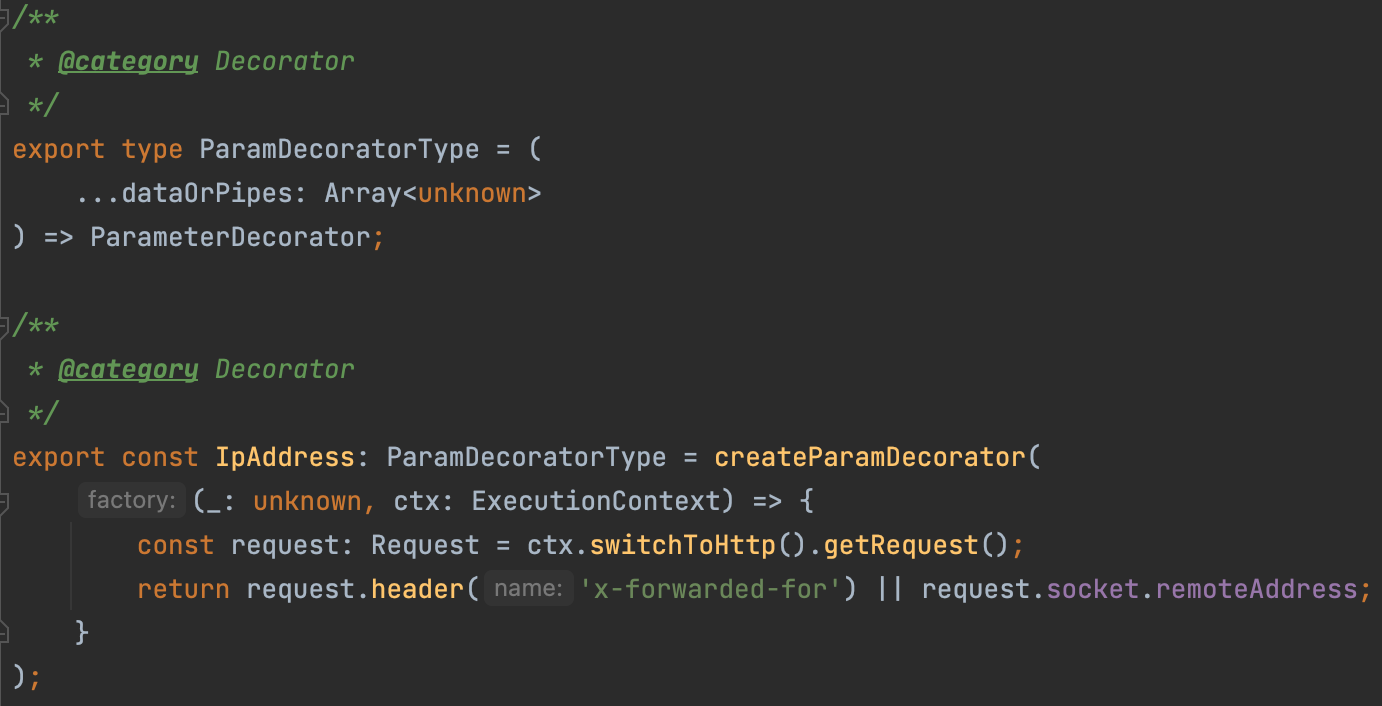
\includegraphics[width=\singlelongfigure]{04/17_node_ip_decorator.png}  
  }
  \caption{Implementarea metodei pentru permis accesul din IntercomService}
\end{figure}

\subsection {Baza de date}

\begin{figure}[h!]
  \centering
  \fbox {
    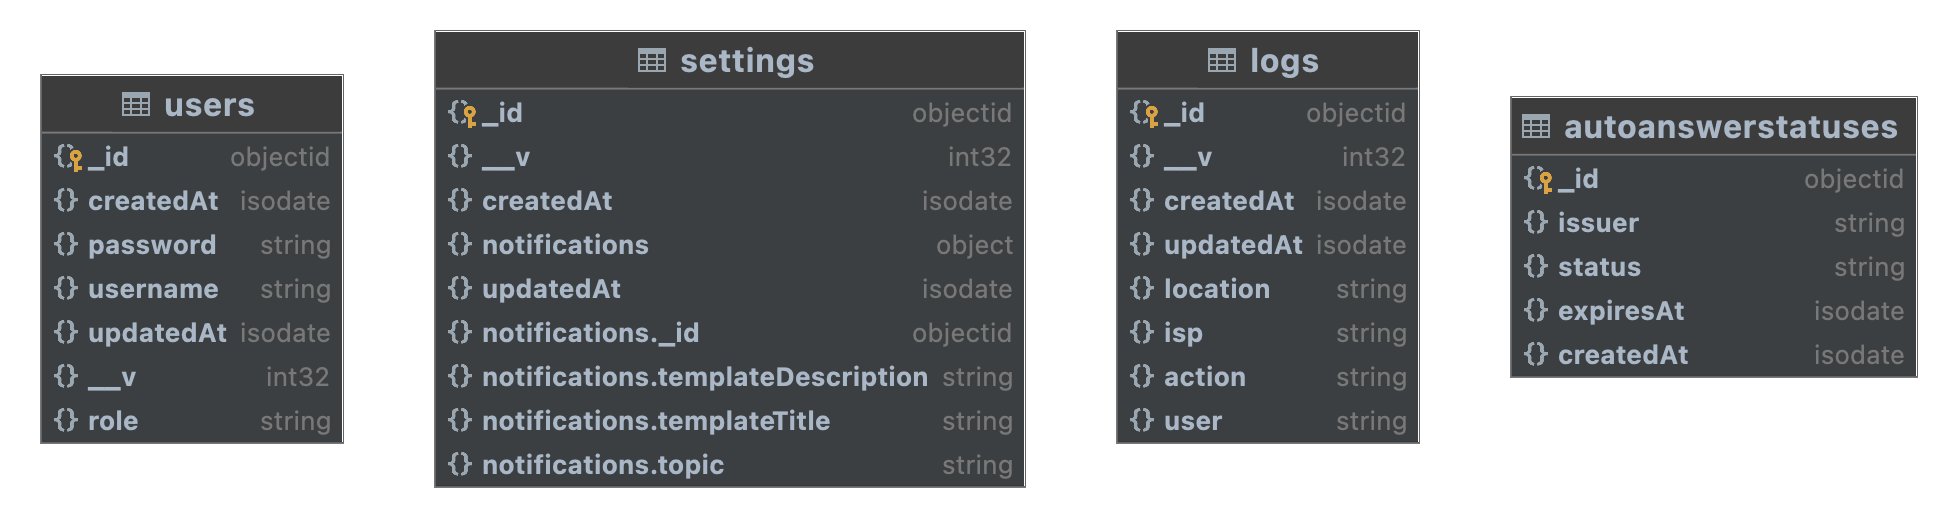
\includegraphics[width=\singlelongfigure]{04/08_schema_db.png}  
  }
  \caption{Schema bazei de date Mongo}
\end{figure}

Baza de date nu oferă nicio rela'tie între documente, însă colec'tia "logs" sau "autoanswerstatuses" trebuie să fie legate din punct de federe logic cu un utilizator. Putem din nou să beneficiem de adnotări, specificând tipul a'steptat pentru validare sau o referin'tă către o alta colec'tie.

Salvăm astfel id-ul utilizatorului care le-a generat împreună cu ele, iar la momentul interogării bazei de date putem folosi metoda "populate()" din driverul Mongoose care va caută modelul pentru adnotări de tip referin'tă. În final, driverul va genera query-uri pentru a aduce referin'tele din colec'tiile corespunzătoare. Dacă o referin'tă nu este găsită, se va întoarce null fiind responsabilitatea aplica'tiei să trateze acest caz. 

\subsection {Aplica'tie mobilă}

Pentru a evita complet problema rulării apelurilor de re'tea pe threadul gre'sit, am folosit un client \acrshort{rest} numit Retrofit, bazat pe OkHttp. Aceasta se ocupă să coordoneze un ThreadPool (o colec'tie de threaduri ce execută taskuri de acela'si tip), astfel că atunci când aplica'tia cheamă un serviciu, se alege unul din threaduri spre a se executa cererea, răspunsul venind sub forma unui callback pe threadul principal.

\begin{figure}[H]
  \centering
  \fbox {
    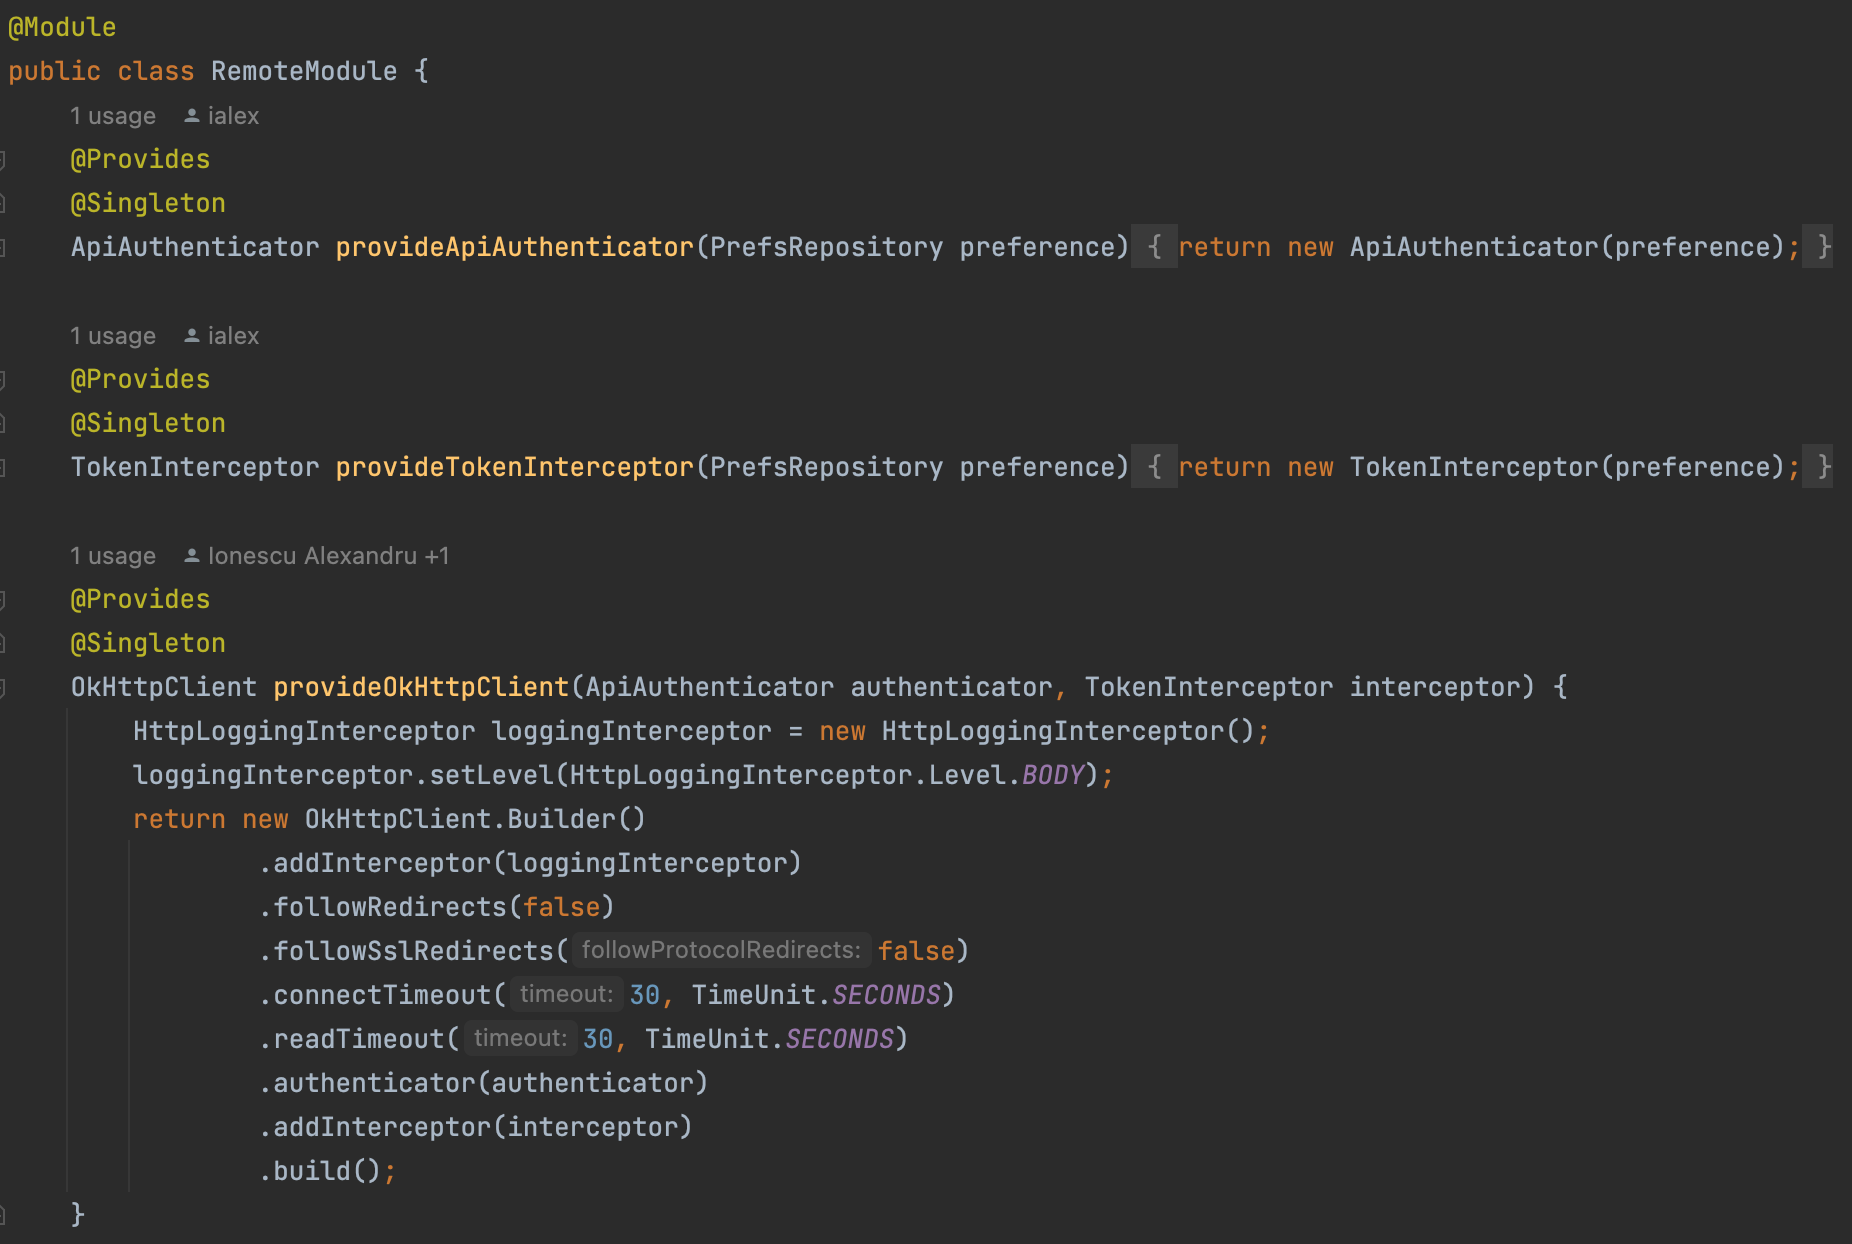
\includegraphics[width=\singlefigure]{04/14_di_network_module.png}  
  }
  \caption{Configurare modul re'tea, împreună cu dependin'tele sale directe}
\end{figure}

Datorită adnotărilor @Singleton toate obiectele din acest modul vor fi instan'tiate o singură dată pe durata aplica'tiei, oferind un punct de acces centralizat pentru toate opera'tiile ce implică chemarea serviciilor \acrshort{rest}.

De asemenea, am configurat Retrofit să folosească Gson pentru serializarea 'si deserializarea \acrshort{dto}-urilor din format \acrshort{json} în instan'te ale claselor din Java. Pentru această opera'tiune se folose'ste de \acrshort{api}-ul reflectiv oferit de limbajul Java spre a chema constructorul implicit al unei clase 'si a seta valorile variabilelor sale.

Urmarind un model \acrshort{mvc} in realizarea aplica'tiei, trebuie sa definim metodele implemenetate de view pentru a fi chemate din interiorul callbackurilor de la nivelul layerului de date. Se decupleaza astfel logica de business de prezentarea interfetei, structura ce faciliteaza testarea si extensibilitatea codului. Cuplarea modulelor trebuie sa fie slaba pentru a evita modificarea excesiva a componentelor cand se schimba specificatiile \cite{sokolova2013android}. 

\begin{figure}[H]
  \centering
  \fbox {
    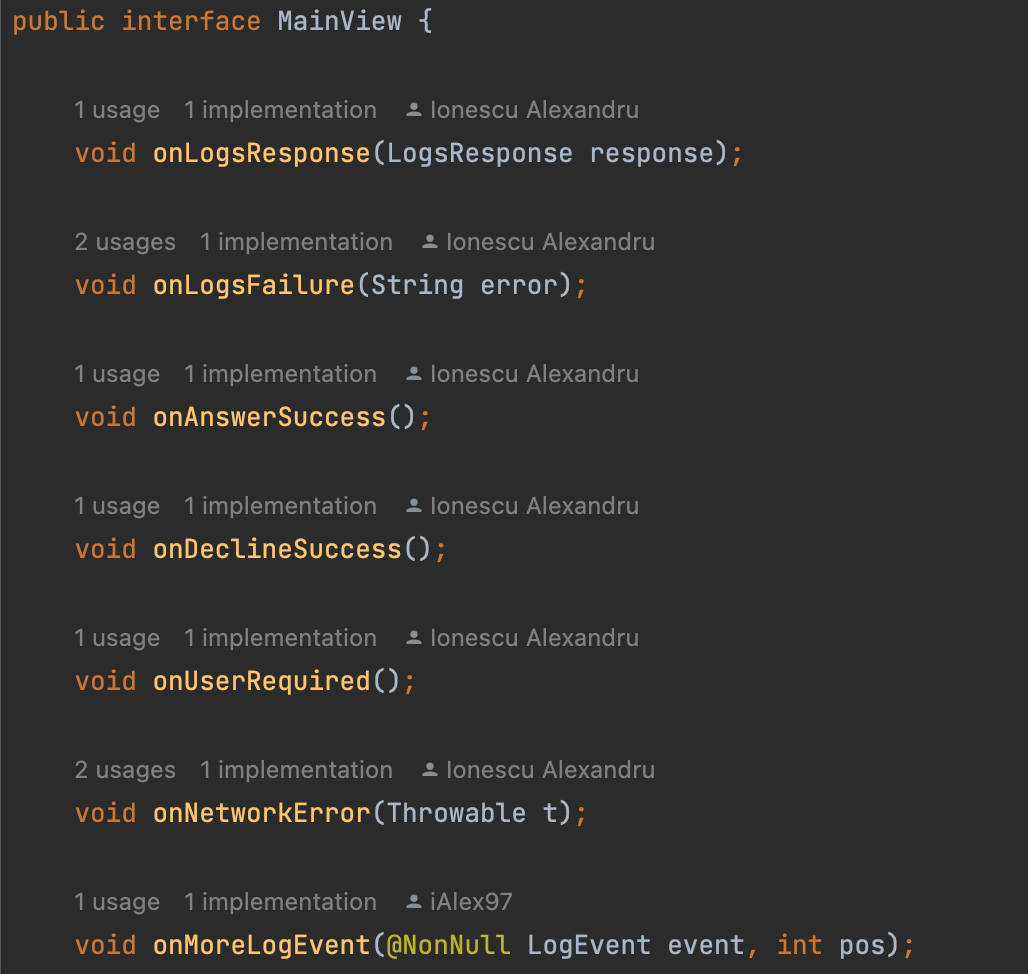
\includegraphics[width=\singlephoto]{04/18_android_main_view.png}
  }
  \caption{Definirea evenimentelor viewului principal}
\end{figure}

\section {Testarea sistemului}

\subsection {Server}

Chiar dacă NestJS oferă suport pentru scrierea de teste unitare prin adăugarea de fisere $.spec.ts$, cea mai mare provocare a fost mockuirea modulului care comunica cu pinii \acrshort{gpio} ai Raspberry Pi. Wrapperul de JavaScript comunică prin intermediul \acrfull{napi} cu o librărie statică ce realizează serializarea 'si deserializarea datelor dintre Node.js/V8 VM 'si C/C++. Această librărie se linkeaza la rândul ei cu $bcm2835$ pentru a ob'tine acces la pinii \acrshort{gpio} 'si alte func'tii din sistemul de \acrfull{io} al cipului Broadcom 2835.

Astfel suntem prezenta'ti cu o problemă, librăria \acrshort{napi} poate fi compilată pe alte arhitecturi, dar cu siguran'tă va genera o excep'tie la rulare când dependin'tă să, $bcm2835$, va încerca să execute instruc'tiuni invalide. Este nevoie de o logică de control care să permită rularea 'si returnarea unor date prestabilite, când se detectează pornirea pe o arhitectura invalidă, cum ar fi în cazul testelor rulate în mod automat prin intermediul pipelineului de integrare continuă.

\subsubsection {Teste unitare}

Următorul pas a fost elaborarea testelor unitare. Prin crearea un fi'sier $.spec.ts$ pentru fiecare controller al API-ului acoperind astfel întreaga func'tionalitate a aplica'tiei. Pentru controllerului responsabil deschiderii interfonului serviciile Firebase 'si baza de date au fost mockuite, testând mecanismul de deschidere/închidere a interfonului în cazul în care aceea'si resursă este accesată de mai mul'ti utilizatori concomitent.

\subsubsection {Teste end-to-end}

Pentru a ne asigura că serviciul \acrshort{rest} răspunde corect se impune necesitatea testelor cap coadă, unde se instantiaza aplica'tia într-o manieră similară produc'tiei, iar cu ajutorul unui client rest se trimit cereri prestabilite 'si se a'steaptă după răspunsurile lor. Astfel parcurgem toată logica serverului, cap-coadă 'si ne vom asigura de un comportament predictibil.

\subsection {Aplica'tia mobilă}

Din cauza fragmentării foarte mari a versiunilor 'si configura'tiilor posibile pentru toate dispozitivele Android pe care ar putea rula aplica'tia, am decis să folosesc "Firebase Test Lab", un serviciu de la Google care oferă posibilitatea rulării unui test automat sau scriptat pe o gamă largă de dispozitive. 
Asigurăm astfel un minim control al calită'tii prin descoperirea timpurie a excep'tiilor netratate.

Tipul de test ales este cel "Robo", care analizează inteligent interfa'ta vizuală a aplica'tiei, după care va genera evenimente de input ca 'si cum ar fi un utilizator. Planul "Spark" de la Firebase ofera acces la 5 rulări pe dispozitive fizice pe zi 'si 10 dispozitive virtuale, deci testele au fost executate în limita acestor constrângeri. 

Pentru a rula un test, trebuie încărcat un APK sau un AAB, ales dispozitivele pentru executarea testului 'si eventualii pa'si adi'tionali pe care îi dorim acoperi'ti de Robo. După introducerea id-ului pentru câmpurile de username 'si parolă împreună cu valorile asociate unui cont de test, acesta reu'sit să se autentifice 'si să facă un stress-test al aplica'tiei. Următoarele dispozitive de test au fost alese:

\begin{itemize}
  \item SM-F926U1, API Level 30 - telefon pliabil, care prezintă o dimensiune non-standard 'si provocări unice în ceea ce prive'ste adaptearea intefetelor pentru o experien'tă cât mai plăcuta
  \item Nexus 5, API Level 23 - versiune mai veche, dar foarte populară de Android, rezolu'tie standard FullHD, acest test se asigura că aplica'tia este compatibilă cu versiuni anterioare ale sistemului de operare
  \item SM-T720, API Level 28 - tabletă, ne asigurăm că aplica'tia este folosibila pe un ecran cu diagonală mare
\end{itemize}

Analizând tabelul pentru performan'tă vizuală, observăm că aplica'tia rulează în margini acceptabile până 'si pe un dispozitiv mai vechi precum Nexus 5.

\begin{table}[ht!]
\begin{tabular}{ll}
\hline
Metrică &  Valoare \\ 
\hline
\hline
Druata până la prima afi'sare & 700ms \\
Eveniment VSync Pierdut & 3\% \\
Laten'ta ridicată input & 0\% \\
Thread UI încet & 4\% \\
Comandă draw înceată & 1\% \\
Încărcare bitmap înceată & 0\% \\
\hline
\end{tabular}
\centering
\caption{Metrice de performan'tă raportate penetru Nexus 5}
\label{tab:metrics}
\end{table}

De asemenea "Test Lab" poate fi chemat din interiorul pipelineul de integrare continuă pentru a rula teste automat după terminarea unui build pe un anumit branch, verificând flow-uri exesitente din aplica'tie împotriva poten'tialelor regresii apărute.

\begin{figure}[h!]
  \centering
  \fbox {
    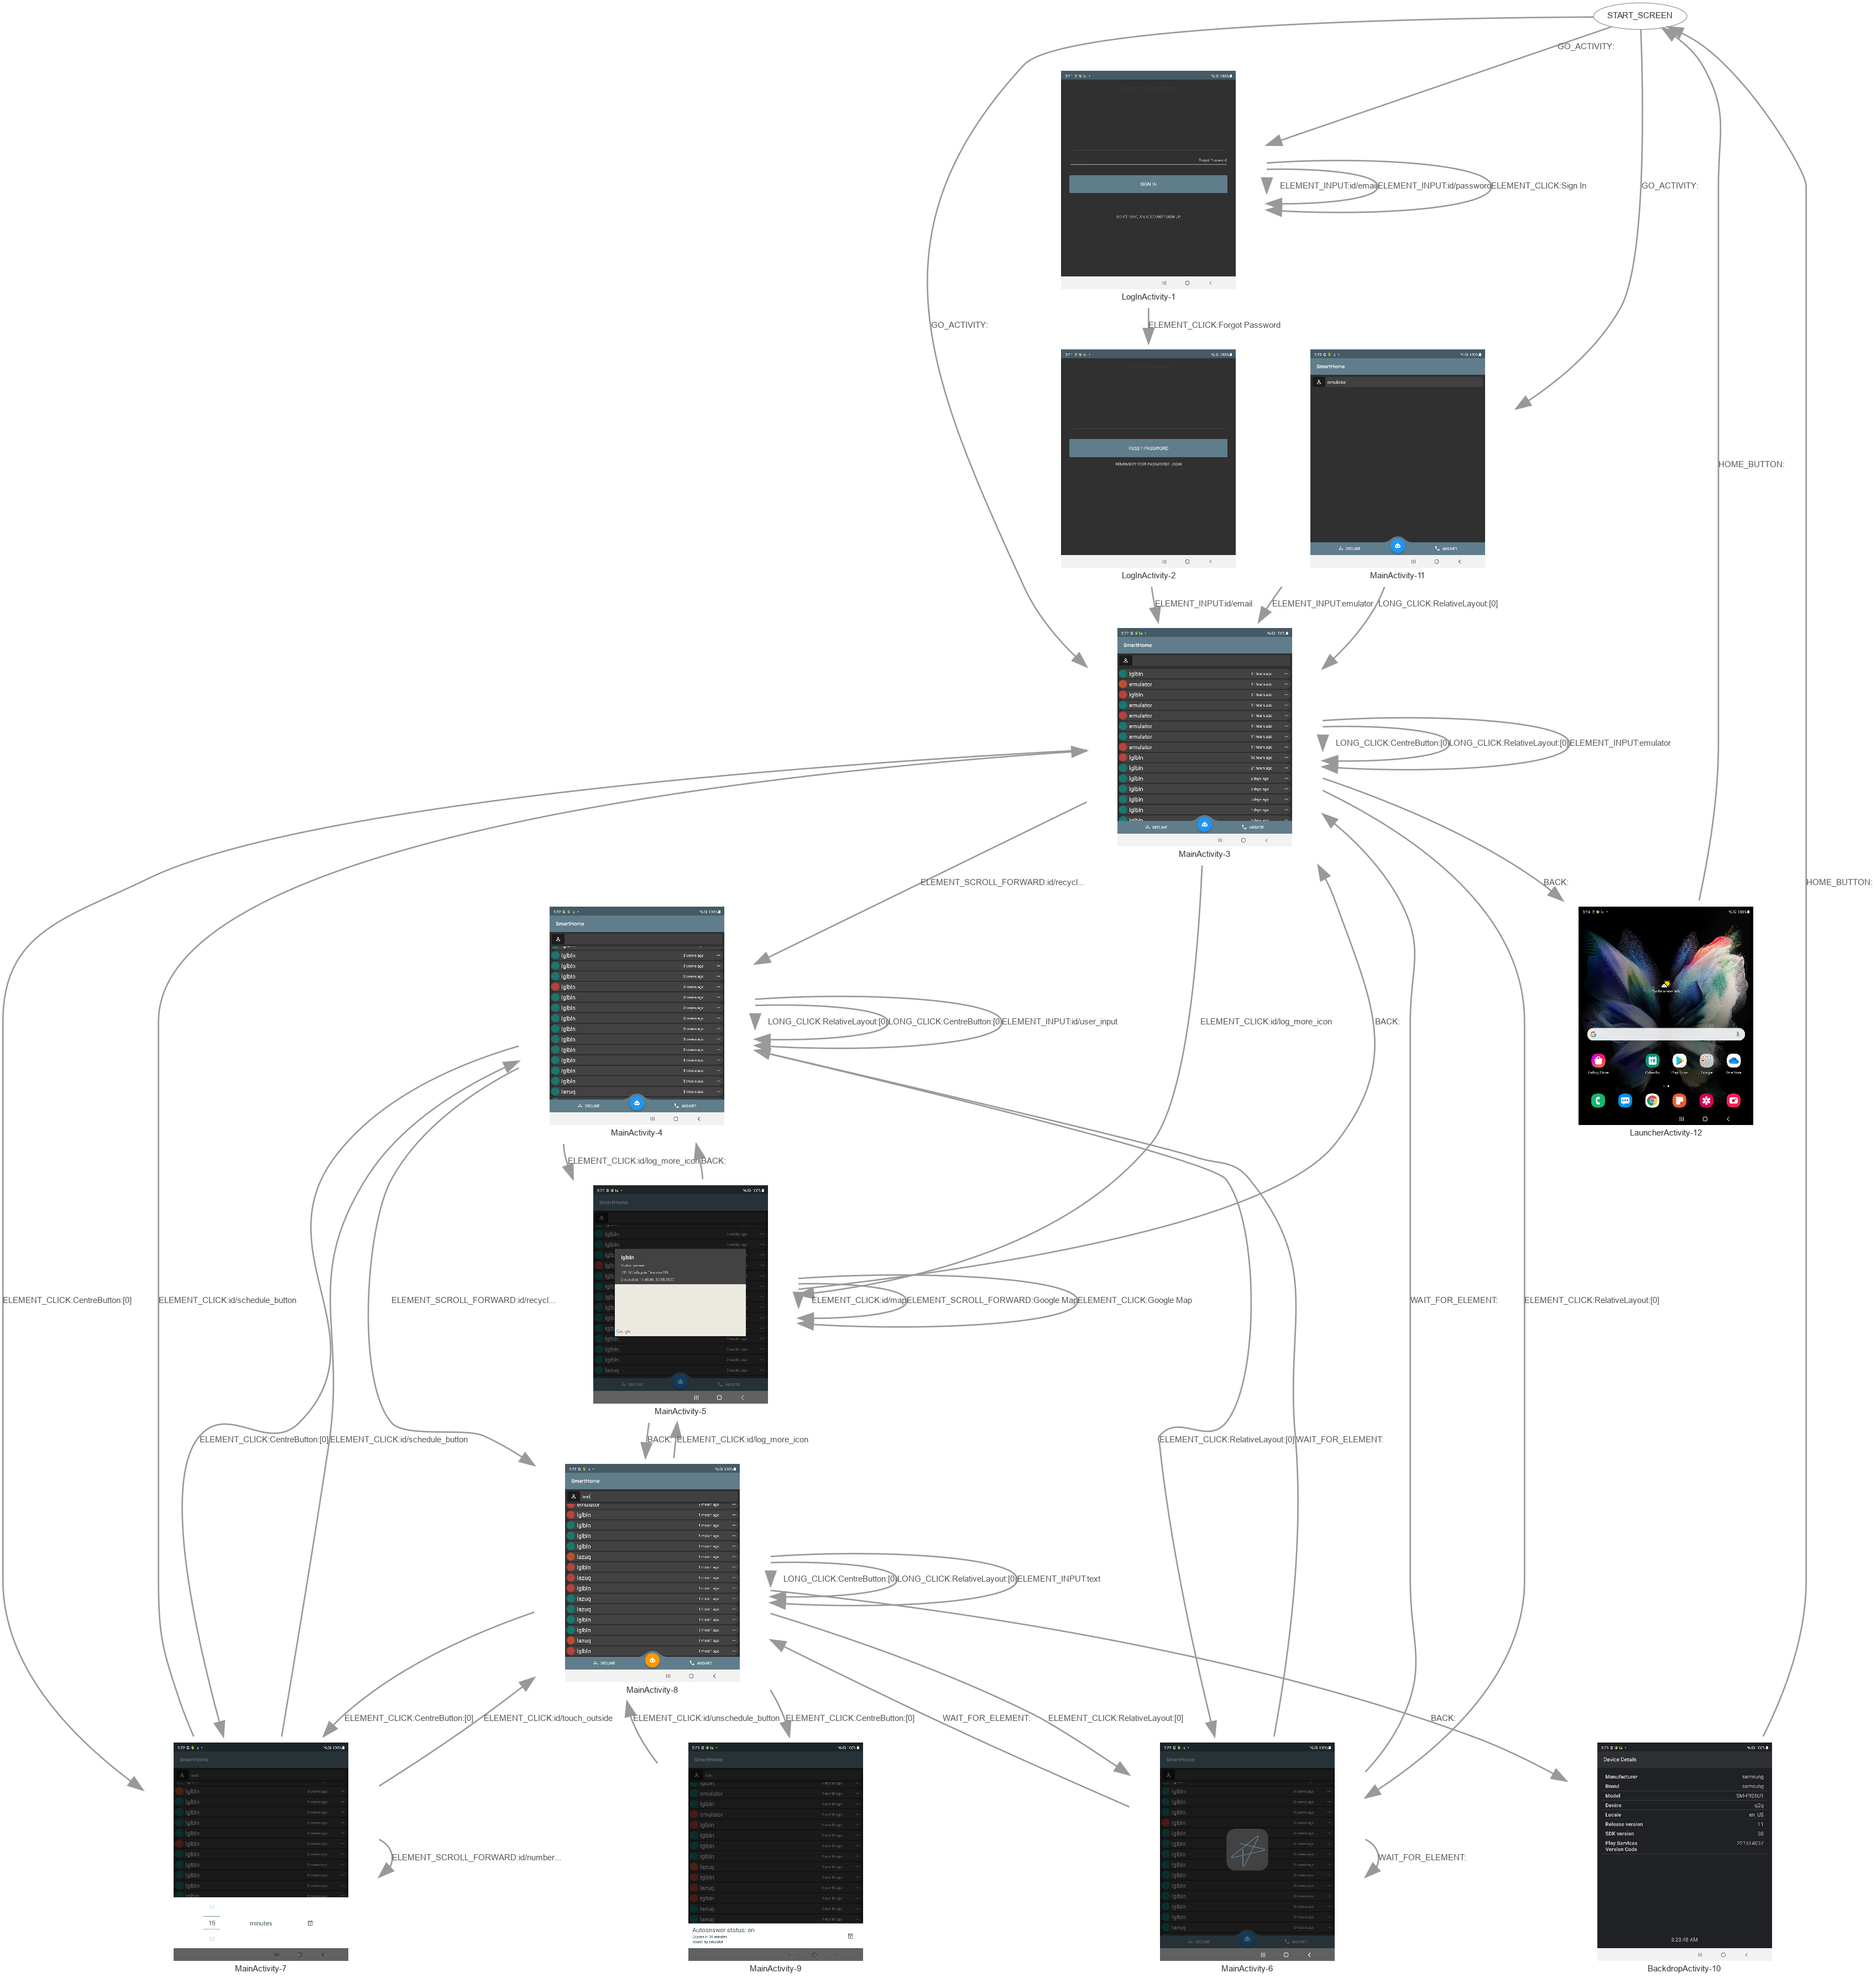
\includegraphics[width=\singlefigure]{04/07_test_lab.png}  
  }
  \caption{Flow testare Robo pe Samsung SM-F926U1}
\end{figure}